% ============================================================
%  Hybrid Pairs Trading Ensemble | 2nd BPS | IIT Bombay
%  Yash Sarang | MS by Research | CMInDS
%  Guide: Prof. Sudeep Bapat
% ============================================================
\documentclass[aspectratio=169,10pt]{beamer}

% ── Core packages ─────────────────────────────────────────
\usepackage[utf8]{inputenc}
\usepackage[T1]{fontenc}
\usepackage{lmodern}
\usepackage{amsmath,amssymb}
\usepackage{graphicx}
\usepackage{booktabs}
\usepackage{xcolor}
\usepackage{colortbl}
\usepackage{tikz}
\usetikzlibrary{shapes.geometric,arrows.meta,positioning,fit,calc,
                shadows.blur,backgrounds,decorations.pathreplacing,matrix}
\usepackage{pgfplots}
\pgfplotsset{compat=1.18}
\usepackage{array}
\usepackage{ragged2e}
\usepackage{hyperref}
\usepackage{multirow}

% ── IITB Brand Colours ────────────────────────────────────
\definecolor{iitbnavy}{RGB}{0,51,102}
\definecolor{iitbsaff}{RGB}{245,124,0}
\definecolor{iitbgold}{RGB}{255,195,0}
\definecolor{iitblt}  {RGB}{230,241,255}
\definecolor{bodytext}{RGB}{30,30,50}
\definecolor{goodgreen}{RGB}{46,139,87}
\definecolor{badred}   {RGB}{205,50,50}
\definecolor{midgray}  {RGB}{120,120,140}
\definecolor{stageone} {RGB}{0,90,160}
\definecolor{stagetwo} {RGB}{160,60,0}
\definecolor{hlrow}    {RGB}{255,243,205}
\definecolor{hlblue}   {RGB}{220,235,255}

% ── Theme ─────────────────────────────────────────────────
\usetheme{default}
\usecolortheme[named=iitbnavy]{structure}
\setbeamertemplate{navigation symbols}{}
\setbeamertemplate{blocks}[rounded][shadow=false]

\setbeamercolor{frametitle}          {bg=iitbnavy, fg=white}
\setbeamercolor{block title}         {bg=iitbnavy, fg=white}
\setbeamercolor{block body}          {bg=iitblt,   fg=bodytext}
\setbeamercolor{block title alerted} {bg=iitbsaff!90, fg=white}
\setbeamercolor{block body alerted}  {bg=iitbsaff!10, fg=bodytext}
\setbeamercolor{alerted text}        {fg=iitbsaff}
\setbeamercolor{section in toc}      {fg=iitbnavy}
\setbeamercolor{item}                {fg=iitbsaff}
\setbeamercolor{subitem}             {fg=iitbnavy}
\setbeamercolor{normal text}         {fg=bodytext}
\setbeamercolor{palette primary}     {bg=iitbnavy,fg=white}

% ── Frametitle ────────────────────────────────────────────
\setbeamertemplate{frametitle}{%
  \nointerlineskip
  \begin{beamercolorbox}[wd=\paperwidth,ht=0.48cm,dp=0.12cm,leftskip=0.45cm]{frametitle}%
    \usebeamerfont{frametitle}\insertframetitle%
  \end{beamercolorbox}%
  \nointerlineskip
  {\color{iitbsaff}\rule{\paperwidth}{1.4pt}}%
  \vspace{0.08cm}%
}

% ── Footline ──────────────────────────────────────────────
\setbeamertemplate{footline}{%
  \leavevmode\hbox{%
    \begin{beamercolorbox}[wd=0.33\paperwidth,ht=0.22cm,dp=0.12cm,leftskip=0.25cm]{palette primary}%
      \tiny\color{white}Yash Sarang (CMInDS, IIT Bombay)%
    \end{beamercolorbox}%
    \begin{beamercolorbox}[wd=0.34\paperwidth,ht=0.22cm,dp=0.12cm,center]{palette primary}%
      \tiny\color{white}Hybrid Pairs Trading Ensemble $|$ 2nd BPS%
    \end{beamercolorbox}%
    \begin{beamercolorbox}[wd=0.33\paperwidth,ht=0.22cm,dp=0.12cm,rightskip=0.25cm]{palette primary}%
      \tiny\color{white}\hfill June 2026\hspace{1em}\insertframenumber\,/\,\inserttotalframenumber%
    \end{beamercolorbox}%
  }%
}

% ── Fonts ─────────────────────────────────────────────────
\setbeamerfont{frametitle}               {size=\small,series=\bfseries}
\setbeamerfont{block title}              {size=\footnotesize,series=\bfseries}
\setbeamerfont{itemize/enumerate body}   {size=\small}
\setbeamerfont{itemize/enumerate subbody}{size=\scriptsize}

% ── Bullets ───────────────────────────────────────────────
\setbeamertemplate{itemize item}  {\color{iitbsaff}\small$\blacktriangleright$}
\setbeamertemplate{itemize subitem}{\color{iitbnavy}\footnotesize$\circ$}
\setbeamertemplate{enumerate item}{\color{iitbnavy}\small\insertenumlabel.}

% ── Margins ───────────────────────────────────────────────
\setbeamersize{text margin left=0.4cm,text margin right=0.4cm}
\setlength{\leftmargini}{1.1em}
\setlength{\leftmarginii}{0.9em}

% ── TikZ node styles ──────────────────────────────────────
\tikzset{
  % Generic coloured box
  fbox/.style={rectangle, rounded corners=3pt, align=center,
               draw=#1!70!black, thick, fill=#1!12,
               font=\scriptsize\bfseries, text=#1!30!black,
               minimum height=0.75cm, minimum width=2.5cm, inner sep=5pt},
  fbox/.default=iitbnavy,
  % Stage-specific variants
  s1box/.style={fbox=stageone},
  s2box/.style={fbox=stagetwo},
  % Highlighted focus box
  focbox/.style={rectangle, rounded corners=4pt, align=center,
                 draw=iitbsaff, very thick, fill=iitbsaff!10,
                 font=\scriptsize\bfseries, text=iitbnavy!80!black,
                 minimum height=0.85cm, minimum width=2.8cm, inner sep=5pt},
  % Output / metric box
  outbox/.style={fbox=goodgreen},
  % Arrows
  arr/.style  ={-{Stealth[length=5pt,width=4pt]}, thick, draw=iitbnavy!65},
  darr/.style ={-{Stealth[length=4pt]}, dashed, thick, draw=midgray},
}

% ── Metadata ─────────────────────────────────────────────
\title[Hybrid Pairs Trading Ensemble $|$ 2nd BPS]{%
  Hybrid Pairs Trading Ensemble:\\%
  \small Pair Selection via ML-Statistical Ensembles on NSE Nifty Equities}
\author[Yash Sarang]{Yash Sarang}
\institute[IIT Bombay]{CMInDS, IIT Bombay}
\date{June 2026}

% ─────────────────────────────────────────────────────────
\begin{document}

%% =========================================================
%% SLIDE 1 — Title
%% =========================================================
\begin{frame}[plain]
  \begin{tikzpicture}[remember picture,overlay]
    \fill[iitbnavy]  (current page.north west)
                     rectangle ([yshift=-0.41\paperheight]current page.north east);
    \fill[iitbsaff]  ([yshift=-0.41\paperheight]current page.north west)
                     rectangle ([yshift=-0.428\paperheight]current page.north east);
    \fill[iitblt!25] ([yshift=-0.428\paperheight]current page.north west)
                     rectangle (current page.south east);
    \fill[iitbsaff!25,opacity=0.35]
         ([xshift=-3.5cm,yshift=-2.2cm]current page.north east) circle(3.0cm);
    \fill[iitbgold!35,opacity=0.25]
         ([xshift=-1.5cm,yshift=-4.2cm]current page.north east) circle(1.8cm);
  \end{tikzpicture}
  \vspace{0.04\paperheight}
  \begin{center}
    {\color{white}\small\bfseries 2nd Bi-Annual Progress Seminar (BPS)}\\[3pt]
    {\color{iitbgold}\rule{0.50\linewidth}{0.8pt}}\\[5pt]
    {\color{white}\large\bfseries Hybrid Pairs Trading Ensemble}\\[2pt]
    {\color{white}\footnotesize Pair Selection via ML-Statistical Ensembles on NSE Nifty Equities}\\[11pt]
    {\color{iitbsaff!60}\rule{0.38\linewidth}{0.5pt}}\\[9pt]
    {\color{iitbnavy}\normalsize\bfseries Yash Sarang}\\[1pt]
    {\color{iitbnavy}\small MS by Research Student (CMInDS)}\\[1pt]
    {\color{iitbnavy}\small Guide: \textbf{Prof.\ Sudeep Bapat}}\\[5pt]
    {\color{iitbnavy!80}\footnotesize Centre for Machine Intelligence \& Data Science, IIT Bombay}\\[2pt]
    {\color{iitbnavy!60}\scriptsize June 2026}
  \end{center}
\end{frame}

%% =========================================================
%% SLIDE 2 — Outline
%% =========================================================
\begin{frame}{Presentation Outline}
  \tableofcontents[hideallsubsections]
\end{frame}

%% =========================================================
\section{The Pairs Trading Problem}
%% =========================================================

%% SLIDE 3 — What is pairs trading?
\begin{frame}{Pairs Trading: Market-Neutral Statistical Arbitrage}
  \begin{columns}[T]
    \begin{column}{0.56\textwidth}
      \textbf{Core Idea}
      \begin{itemize}\itemsep4pt
        \item Identify two historically co-moving stocks whose spread has temporarily diverged.
        \item \emph{Long} the underpriced leg, \emph{Short} the overpriced leg.
        \item Profit when spread mean-reverts. \textbf{Broad market exposure cancels} $\to$ market neutral.
      \end{itemize}
      \vspace{5pt}
      \textbf{Why NSE is Especially Challenging}
      \begin{itemize}\itemsep3pt
        \item India-specific frictions: STT (sell-side), stamp duty, exchange fees, GST.
        \item Total round-trip cost: \alert{\textbf{16.28 bps per pair trade}}.
        \item Strategy must generate gross alpha \emph{consistently} above this threshold.
      \end{itemize}
    \end{column}
    \begin{column}{0.41\textwidth}
      \begin{block}{NSE Transaction Cost Breakdown}
        \centering\scriptsize
        \renewcommand{\arraystretch}{1.3}
        \begin{tabular}{lc}
          \toprule
          \textbf{Cost Component} & \textbf{bps} \\
          \midrule
          STT (sell-side only)    & 10.00 \\
          Stamp Duty (buy-side)   & 1.50  \\
          Exchange / SEBI fee     & 0.33  \\
          GST on charges          & 0.06  \\
          Conservative Slippage   & 2.00  \\
          \midrule
          \textbf{Total Round-Trip} & \textbf{\alert{16.28}} \\
          \bottomrule
        \end{tabular}
      \end{block}
    \end{column}
  \end{columns}
\end{frame}

%% SLIDE 4 — Two-stage framing  (FIXED: no \color inside TikZ text; use label nodes outside)
\begin{frame}{Pairs Trading is a Two-Stage Problem}
  \vspace{2pt}
  \begin{center}
  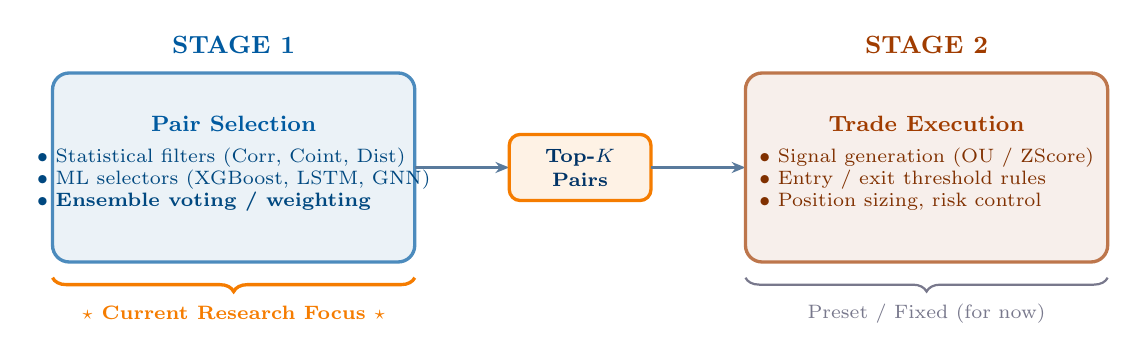
\begin{tikzpicture}[x=1cm,y=1cm]

    % ── Stage 1 rectangle ──────────────────────────────────
    \draw[stageone!70,very thick,rounded corners=6pt,fill=stageone!8]
          (-0.6,-1.2) rectangle (4.0,1.2);
    \node[font=\small\bfseries,text=stageone] at (1.7, 1.55) {STAGE 1};
    \node[font=\footnotesize\bfseries,text=stageone] at (1.7, 0.55)
          {Pair Selection};
    \node[font=\scriptsize,text=stageone!80!black,align=left] at (1.7,-0.15)
          {$\bullet$ Statistical filters (Corr, Coint, Dist)\\
           $\bullet$ ML selectors (XGBoost, LSTM, GNN)\\
           $\bullet$ \textbf{Ensemble voting / weighting}};

    % ── Focus brace under Stage 1 ──────────────────────────
    \draw[iitbsaff,very thick,decorate,
          decoration={brace,amplitude=5pt,mirror}]
          (-0.6,-1.4) -- (4.0,-1.4);
    \node[font=\scriptsize\bfseries,text=iitbsaff] at (1.7,-1.85)
          {$\star$\ Current Research Focus\ $\star$};

    % ── Arrow + Top-K node ─────────────────────────────────
    \draw[arr] (4.0,0) -- (5.2,0);
    \draw[focbox] (5.2,-0.42) rectangle (7.0,0.42);
    \node[font=\scriptsize\bfseries,text=iitbnavy] at (6.1,0.12) {Top-$K$};
    \node[font=\scriptsize\bfseries,text=iitbnavy] at (6.1,-0.15) {Pairs};

    % ── Arrow ─────────────────────────────────────────────
    \draw[arr] (7.0,0) -- (8.2,0);

    % ── Stage 2 rectangle ──────────────────────────────────
    \draw[stagetwo!70,very thick,rounded corners=6pt,fill=stagetwo!8]
          (8.2,-1.2) rectangle (12.8,1.2);
    \node[font=\small\bfseries,text=stagetwo] at (10.5, 1.55) {STAGE 2};
    \node[font=\footnotesize\bfseries,text=stagetwo] at (10.5, 0.55)
          {Trade Execution};
    \node[font=\scriptsize,text=stagetwo!80!black,align=left] at (10.5,-0.15)
          {$\bullet$ Signal generation (OU / ZScore)\\
           $\bullet$ Entry / exit threshold rules\\
           $\bullet$ Position sizing, risk control};

    % ── "Fixed" brace under Stage 2 ───────────────────────
    \draw[midgray,thick,decorate,
          decoration={brace,amplitude=5pt,mirror}]
          (8.2,-1.4) -- (12.8,-1.4);
    \node[font=\scriptsize,text=midgray] at (10.5,-1.85)
          {Preset / Fixed (for now)};

  \end{tikzpicture}
  \end{center}
  \vspace{6pt}
  \small\textbf{Research Strategy:} Stage 2 is \alert{frozen} at its best empirical configuration so that all Stage 1 ensemble experiments are directly comparable.
\end{frame}

%% =========================================================
\section{Data \& Universe Decisions}
%% =========================================================

%% SLIDE 5 — Data decisions
\begin{frame}{Data \& Universe: Key Design Decisions}
  \begin{columns}[T]
    \begin{column}{0.54\textwidth}
      \textbf{Decision 1 --- Universe: Nifty 100 (Primary)}
      \begin{itemize}\itemsep2pt
        \item 89 liquid tickers after survivorship-bias filtering.
        \item $C(89,2) = 3{,}916$ candidate pairs per fold.
        \item Broader universe $\to$ more candidates but noisier co-movements.
      \end{itemize}
      \vspace{5pt}
      \textbf{Decision 2 --- Frequency: Daily (1D) over Hourly (1H)}
      \begin{itemize}\itemsep2pt
        \item Hourly data contains severe microstructure noise.
        \item Hurst exponent: hourly $\approx 0.251$ vs.\ daily $\approx 0.190$ (daily more mean-reverting).
        \item Hourly $\to$ 904 trades/yr $\to$ \alert{bankruptcy} under 16.28 bps.
      \end{itemize}
      \vspace{5pt}
      \textbf{Decision 3 --- Validation: Expanding WFV}
      \begin{itemize}\itemsep2pt
        \item 6 folds, each extending training window from 2015 onward.
        \item Avoids look-ahead bias; mimics live trading regime.
      \end{itemize}
    \end{column}
    \begin{column}{0.43\textwidth}
      \begin{block}{E1: Daily vs.\ Hourly (No Hold Limit)}
        \centering\scriptsize
        \renewcommand{\arraystretch}{1.2}
        \begin{tabular}{lcc}
          \toprule
          \textbf{Metric} & \textbf{Daily} & \textbf{Hourly} \\
          \midrule
          Gross Sharpe   & 1.144 & 0.488 \\
          Gross Ann. Ret & 5.0\% & 1.3\% \\
          Net Sharpe     & \textcolor{badred}{$-2.29$} & \textcolor{badred}{$-6.55$} \\
          Net Ann. Ret   & $-11.3\%$ & \alert{Bankrupt} \\
          Net Max DD     & 29.9\% & 214\% \\
          Trades / yr    & 673   & 904 \\
          \bottomrule
        \end{tabular}
      \end{block}
      \vspace{4pt}
      \begin{block}{Expanding WFV Fold Structure}
        \centering\scriptsize
        \renewcommand{\arraystretch}{1.2}
        \begin{tabular}{ccc}
          \toprule
          \textbf{Fold} & \textbf{Train} & \textbf{OOS Test} \\
          \midrule
          F1 & 2015--17 & 2018 \\
          F2 & 2015--18 & 2019 \\
          F3 & 2015--19 & 2020 \\
          F4 & 2015--20 & 2021 \\
          F5 & 2015--21 & 2022 \\
          F6 & 2015--22 & 2023--24 \\
          \bottomrule
        \end{tabular}
      \end{block}
    \end{column}
  \end{columns}
\end{frame}

%% =========================================================
\section{Stage 2: The Preset Execution Engine}
%% =========================================================

%% SLIDE 6 — Stage 2 in detail
\begin{frame}{Stage 2 (Preset \& Fixed): The Execution Engine}
  \small\textbf{Context:} Stage 2 is \emph{not} the experimental variable. It is frozen at the best configuration found to make all Stage 1 comparisons apples-to-apples.
  \vspace{4pt}
  \begin{columns}[T]
    \begin{column}{0.54\textwidth}
      \textbf{Signal Model: Ornstein-Uhlenbeck (OU) Threshold}
      \begin{itemize}\itemsep3pt
        \item Spread $x_t$ modeled as: $dx_t = \kappa(\theta - x_t)\,dt + \sigma\,dW_t$
        \item Parameters $(\kappa, \theta, \sigma)$ estimated via MLE on each training fold.
        \item Z-score: $z_t = (x_t - \theta) / \sigma_{\mathrm{OU}}$
        \item \textbf{Entry:} $|z_t|>2.0$ \quad \textbf{Exit:} $|z_t|<0.5$ \quad \textbf{Stop:} $|z_t|>3.0$
      \end{itemize}
      \vspace{4pt}
      \textbf{Why OU over ZScore / Kalman / MLSignal?}
      \begin{itemize}\itemsep2pt
        \item ZScore triggers too many trades (no half-life awareness).
        \item MLSignal and Kalman both over-trade under 16.28 bps costs.
        \item OU is the \emph{only} signal surviving post-cost.
      \end{itemize}
    \end{column}
    \begin{column}{0.43\textwidth}
      \begin{block}{Fixed Backtest Parameters}
        \centering\scriptsize
        \renewcommand{\arraystretch}{1.3}
        \begin{tabular}{lc}
          \toprule
          \textbf{Parameter} & \textbf{Fixed Value} \\
          \midrule
          Signal Warmup      & 126 trading days \\
          Entry threshold    & $|z|>2.0$ \\
          Exit threshold     & $|z|<0.5$ \\
          Hard stop-loss     & $|z|>3.0$ \\
          \rowcolor{hlrow} Min Hold Period & \textbf{30 trading days} \\
          Max Active Pairs   & 10 \\
          Capital per pair   & INR 1,00,000 \\
          Total Capital      & INR 10,00,000 \\
          Transaction Costs  & 16.28 bps (full) \\
          Execution Mode     & CPU-only (deterministic) \\
          \bottomrule
        \end{tabular}
      \end{block}
    \end{column}
  \end{columns}
\end{frame}

%% SLIDE 7 — Why 30 days?
\begin{frame}{Why the 30-Day Minimum Hold Period?}
  \begin{columns}[T]
    \begin{column}{0.54\textwidth}
      \textbf{Cost Survival Requires Limiting Turnover}
      \begin{itemize}\itemsep4pt
        \item Without a hold floor, the strategy generates excessive round-trips.
        \item Each exit-and-reentry costs 16.28 bps --- losses compound rapidly.
        \item Optimal hold maps to the OU \emph{spread half-life}:
        \[
          \tau_{1/2} \;=\; \frac{\ln 2}{\kappa} \;\approx\; 20\text{--}30\text{ days}
        \]
        \item Holding beyond 30 days (e.g., 40d) overshoots mean reversion, turning winners into losers.
      \end{itemize}
    \end{column}
    \begin{column}{0.43\textwidth}
      \begin{block}{E2: Hold Period Sweep (stat\_only)}
        \centering\scriptsize
        \renewcommand{\arraystretch}{1.25}
        \begin{tabular}{cccc}
          \toprule
          \textbf{Hold (d)} & \textbf{Gross SR} & \textbf{Net SR} & \textbf{MaxDD} \\
          \midrule
          0  & 0.83 & $-1.89$ & 175.9\% \\
          10 & 0.77 & $-0.20$ & 37.7\%  \\
          20 & 0.70 & $+0.09$ & 20.1\%  \\
          \rowcolor{hlrow}\textbf{30} & \textbf{0.96}
               & \textbf{\color{goodgreen}+0.48} & \textbf{8.2\%} \\
          40 & 0.16 & $-0.24$ & 44.0\%  \\
          \bottomrule
        \end{tabular}
      \end{block}
      \vspace{5pt}
      \small\textbf{Takeaway:} 30 days is the \alert{only configuration} with a positive net Sharpe ratio.
    \end{column}
  \end{columns}
\end{frame}

%% =========================================================
\section{Stage 1: Pair Selection Ensemble Framework}
%% =========================================================

%% SLIDE 8 — All 7 selector models
\begin{frame}{Stage 1: Seven Active Selector Models}
  \vspace{2pt}
  \begin{columns}[T]
    \begin{column}{0.50\textwidth}
      \begin{block}{\color{white}Statistical Selectors (4)}
        \scriptsize\renewcommand{\arraystretch}{1.3}
        \begin{tabular}{>{\bfseries}lp{4.8cm}}
          \toprule
          Selector & Core Metric \\
          \midrule
          Correlation  & Rolling Pearson $\rho$ of log-returns \\
          Distance     & Gatev (2006) normalized SSD of price paths \\
          Cointegration & Engle-Granger two-step ADF p-value \\
          Combined     & Linear composite: Corr + Dist + Coint \\
          \bottomrule
        \end{tabular}
      \end{block}
    \end{column}
    \begin{column}{0.48\textwidth}
      \begin{block}{\color{white}ML Selectors (3 active, 2 disabled)}
        \scriptsize\renewcommand{\arraystretch}{1.3}
        \begin{tabular}{>{\bfseries}lp{4.4cm}}
          \toprule
          Selector & Model / Signal \\
          \midrule
          XGBoost   & Classifier on rolling spread features \\
          LSTM      & Autoencoder reconstruction error \\
          Transformer & Attention-based pair-score output \\
          \midrule
          \textit{GNN}  & \textit{Tested; underperformed} \\
          \textit{CNN}  & \textit{Disabled --- ablation collapse} \\
          \bottomrule
        \end{tabular}
      \end{block}
    \end{column}
  \end{columns}
  \vspace{5pt}
  \small\textbf{Scoring Protocol:} Each selector independently scores all $3{,}916$ pairs. Scores are normalized to $[0,1]$ and combined via \textbf{weighted voting}. Top-$K{=}10$ pairs proceed to Stage 2.
\end{frame}

%% SLIDE 9 — Full pipeline diagram (FIXED: flat left-to-right layout, no relative positioning issues)
\begin{frame}{Full System Architecture: Stage 1 $\to$ Stage 2}
  \vspace{-2pt}
  \begin{center}
  \resizebox{0.97\textwidth}{!}{%
  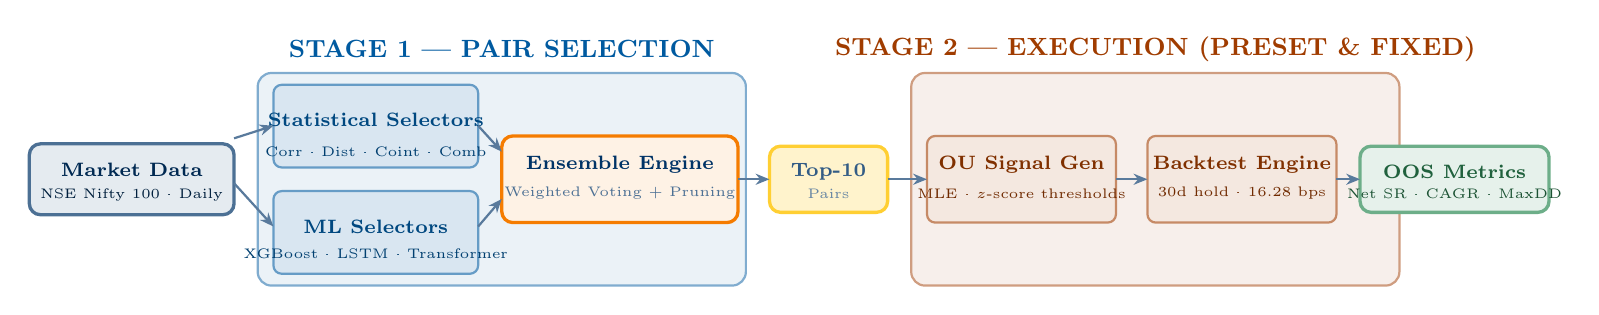
\begin{tikzpicture}[x=1cm,y=1cm]

    %% ── Data ───────────────────────────────────────────────
    \draw[iitbnavy!70,very thick,rounded corners=4pt,fill=iitbnavy!10]
         (0,-0.45) rectangle (2.6,0.45);
    \node[font=\scriptsize\bfseries,text=iitbnavy!80!black,align=center]
         at (1.3,0.12) {Market Data};
    \node[font=\tiny,text=iitbnavy!60!black] at (1.3,-0.20) {NSE Nifty 100 · Daily};

    %% ── Stage 1 background ─────────────────────────────────
    \begin{scope}[on background layer]
      \fill[stageone!8,rounded corners=5pt] (2.9,-1.35) rectangle (9.1,1.35);
      \draw[stageone!50,thick,rounded corners=5pt] (2.9,-1.35) rectangle (9.1,1.35);
    \end{scope}
    \node[font=\small\bfseries,text=stageone] at (6.0,1.65) {STAGE 1 — PAIR SELECTION};

    %% Stat selectors
    \draw[stageone!60,thick,rounded corners=3pt,fill=stageone!15]
         (3.1,0.15) rectangle (5.7,1.20);
    \node[font=\scriptsize\bfseries,text=stageone!80!black,align=center]
         at (4.4,0.75) {Statistical Selectors};
    \node[font=\tiny,text=stageone!70!black] at (4.4,0.35) {Corr · Dist · Coint · Comb};

    %% ML selectors
    \draw[stageone!60,thick,rounded corners=3pt,fill=stageone!15]
         (3.1,-1.20) rectangle (5.7,-0.15);
    \node[font=\scriptsize\bfseries,text=stageone!80!black,align=center]
         at (4.4,-0.60) {ML Selectors};
    \node[font=\tiny,text=stageone!70!black] at (4.4,-0.95) {XGBoost · LSTM · Transformer};

    %% Ensemble engine
    \draw[iitbsaff,very thick,rounded corners=4pt,fill=iitbsaff!10]
         (6.0,-0.55) rectangle (9.0,0.55);
    \node[font=\scriptsize\bfseries,text=iitbnavy,align=center]
         at (7.5,0.18) {Ensemble Engine};
    \node[font=\tiny,text=iitbnavy!70] at (7.5,-0.18) {Weighted Voting + Pruning};

    %% Top-K
    \draw[iitbgold!80,very thick,rounded corners=4pt,fill=iitbgold!20]
         (9.4,-0.42) rectangle (10.9,0.42);
    \node[font=\scriptsize\bfseries,text=iitbnavy!80,align=center]
         at (10.15,0.10) {Top-10};
    \node[font=\tiny,text=iitbnavy!60] at (10.15,-0.18) {Pairs};

    %% ── Stage 2 background ─────────────────────────────────
    \begin{scope}[on background layer]
      \fill[stagetwo!8,rounded corners=5pt] (11.2,-1.35) rectangle (17.4,1.35);
      \draw[stagetwo!50,thick,rounded corners=5pt] (11.2,-1.35) rectangle (17.4,1.35);
    \end{scope}
    \node[font=\small\bfseries,text=stagetwo] at (14.3,1.65)
          {STAGE 2 — EXECUTION (PRESET \& FIXED)};

    %% OU signal
    \draw[stagetwo!60,thick,rounded corners=3pt,fill=stagetwo!12]
         (11.4,-0.55) rectangle (13.8,0.55);
    \node[font=\scriptsize\bfseries,text=stagetwo!80!black,align=center]
         at (12.6,0.18) {OU Signal Gen};
    \node[font=\tiny,text=stagetwo!70!black] at (12.6,-0.18) {MLE · $z$-score thresholds};

    %% Backtest
    \draw[stagetwo!60,thick,rounded corners=3pt,fill=stagetwo!12]
         (14.2,-0.55) rectangle (16.6,0.55);
    \node[font=\scriptsize\bfseries,text=stagetwo!80!black,align=center]
         at (15.4,0.18) {Backtest Engine};
    \node[font=\tiny,text=stagetwo!70!black] at (15.4,-0.18) {30d hold · 16.28 bps};

    %% Output
    \draw[goodgreen!70,very thick,rounded corners=4pt,fill=goodgreen!12]
         (16.9,-0.42) rectangle (19.3,0.42);
    \node[font=\scriptsize\bfseries,text=goodgreen!70!black,align=center]
         at (18.1,0.10) {OOS Metrics};
    \node[font=\tiny,text=goodgreen!60!black] at (18.1,-0.18) {Net SR · CAGR · MaxDD};

    %% ── Arrows ─────────────────────────────────────────────
    \draw[arr] (2.6, 0.52) -- (3.1, 0.68);
    \draw[arr] (2.6,-0.05) -- (3.1,-0.60);
    \draw[arr] (5.7, 0.68) -- (6.0, 0.35);
    \draw[arr] (5.7,-0.60) -- (6.0,-0.25);
    \draw[arr] (9.0, 0) -- (9.4, 0);
    \draw[arr] (10.9,0) -- (11.4,0);
    \draw[arr] (13.8,0) -- (14.2,0);
    \draw[arr] (16.6,0) -- (16.9,0);

  \end{tikzpicture}
  }
  \end{center}
  \vspace{2pt}
  \centering\scriptsize\color{midgray}
  6 expanding WFV folds $\cdot$ All metrics OOS $\cdot$ Stage 2 parameters \textbf{frozen} across all Stage 1 experiments
\end{frame}

%% =========================================================
\section{Ablation Results: Standalone Selectors}
%% =========================================================

%% SLIDE 10 — Standalone ablation with bar chart
\begin{frame}{Ablation: Standalone Selectors (Fixed Stage 2 = OU)}
  \begin{columns}[T]
    \begin{column}{0.46\textwidth}
      \begin{block}{E3/E4.S: Standalone OOS Net Sharpe Ratios}
        \centering\scriptsize\renewcommand{\arraystretch}{1.3}
        \begin{tabular}{lccc}
          \toprule
          \textbf{Selector} & \textbf{Gross SR} & \textbf{Net SR} & \textbf{CAGR} \\
          \midrule
          \rowcolor{hlrow}\textbf{Distance} & \textbf{1.022} & \textbf{\color{goodgreen}+0.829} & +9.1\% \\
          XGBoost (ML) & 0.399 & \color{goodgreen}+0.610 & +6.6\% \\
          LSTM         & 0.727 & \color{goodgreen}+0.356 & +3.2\% \\
          Cointegration & 0.181 & \color{goodgreen}+0.167 & +1.0\% \\
          Correlation  & 0.435 & \color{goodgreen}+0.160 & +1.5\% \\
          Combined     & 0.282 & $-0.092$ & $-0.9\%$ \\
          Transformer  & 0.053 & $-0.380$ & $-3.7\%$ \\
          GNN          & $-0.091$ & \color{badred}$-0.415$ & $-4.3\%$ \\
          \midrule
          \textbf{Equal-Weight All} & $-0.256$
               & \color{badred}\textbf{$-0.719$} & $-8.1\%$ \\
          \bottomrule
        \end{tabular}
      \end{block}
    \end{column}
    \begin{column}{0.52\textwidth}
      \vspace{2pt}
      \resizebox{\columnwidth}{!}{%
      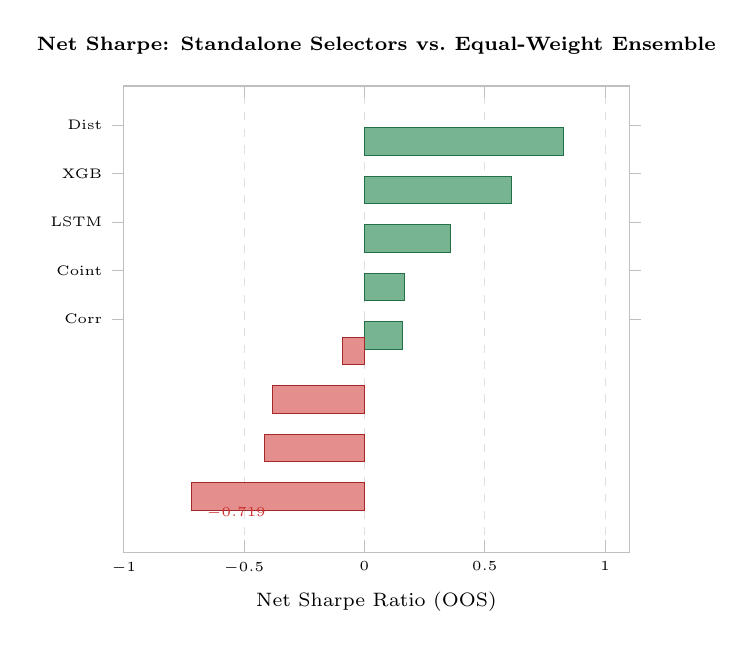
\begin{tikzpicture}
        \begin{axis}[
          xbar, xmin=-1.0, xmax=1.1,
          width=8cm, height=7.5cm,
          bar width=0.35cm,
          symbolic y coords={EqWt-All,GNN,Trans,Comb,Corr,Coint,LSTM,XGB,Dist},
          ytick=data,
          yticklabel style={font=\tiny},
          xticklabel style={font=\tiny},
          xlabel={\scriptsize Net Sharpe Ratio (OOS)},
          xlabel style={font=\scriptsize},
          xtick={-1.0,-0.5,0,0.5,1.0},
          xmajorgrids=true,grid style={dashed,gray!25},
          axis line style={gray!50},
          tick style={gray!50},
          title={\scriptsize Net Sharpe: Standalone Selectors vs.\ Equal-Weight Ensemble},
          title style={font=\scriptsize\bfseries,yshift=2pt},
        ]
          % Positive bars green, negative red
          \addplot[fill=goodgreen!65,draw=goodgreen!80!black]
            coordinates {(0.829,Dist)(0.610,XGB)(0.356,LSTM)(0.167,Coint)(0.160,Corr)};
          \addplot[fill=badred!55,draw=badred!80!black]
            coordinates {(-0.092,Comb)(-0.380,Trans)(-0.415,GNN)(-0.719,EqWt-All)};
          % Annotation for worst bar
          \node[font=\tiny\bfseries,text=badred] at (axis cs:-0.719,EqWt-All)
               [xshift=2pt,right] {$-0.719$};
        \end{axis}
      \end{tikzpicture}
      }
    \end{column}
  \end{columns}
\end{frame}

%% =========================================================
\section{Ablation Results: Ensemble Experiments}
%% =========================================================

%% SLIDE 11 — Dilution paradox explained
\begin{frame}{The Ensemble Dilution Paradox}
  \vspace{2pt}
  \begin{columns}[T]
    \begin{column}{0.52\textwidth}
      \textbf{Naive Equal-Weight Ensemble of All 8 Selectors}
      \begin{itemize}\itemsep4pt
        \item Each selector weight: $w_i = 1/8$.
        \item \alert{\textbf{Result: Net SR collapses from +0.829 to $-0.719$.}}
        \item Distance (+0.829) and XGBoost (+0.610) are \emph{individually} profitable --- yet their combination with GNN/Transformer destroys the strategy.
      \end{itemize}
      \vspace{5pt}
      \textbf{Why Dilution Happens}
      \begin{itemize}\itemsep4pt
        \item GNN and Transformer nominate ``false'' pairs (negative alpha) that contaminate the Top-$K$.
        \item Even 2--3 bad pairs out of 10 active positions can flip the portfolio negative.
        \item \textbf{Insight:} Selection \emph{quality} dominates model \emph{count}.
      \end{itemize}
    \end{column}
    \begin{column}{0.45\textwidth}
      \vspace{4pt}
      \begin{center}
      \resizebox{\columnwidth}{!}{%
      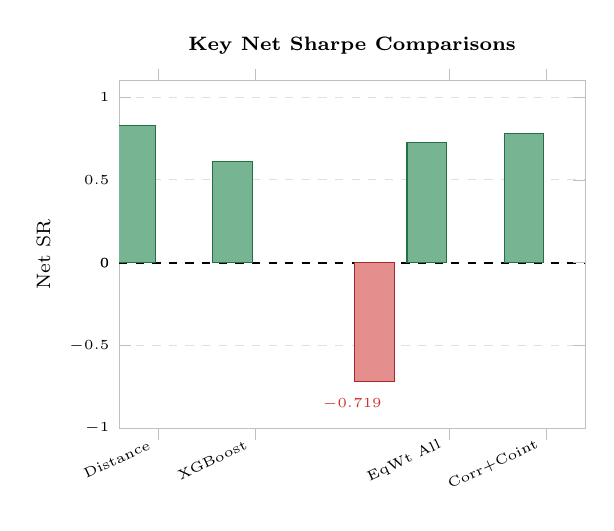
\begin{tikzpicture}[x=1cm,y=1cm]
        % Visual: waterfall / comparison
        % Bars: Dist, XGB, Equal, Corr+Coint, ConfigC
        \begin{axis}[
          ybar, ymin=-1.0, ymax=1.1,
          width=7.5cm, height=6cm,
          bar width=0.5cm,
          symbolic x coords={Dist,XGB,EqWt,Corr+Coint,Cfg-C},
          xtick=data,
          xticklabels={Distance,XGBoost,EqWt All,Corr+Coint,Config C},
          xticklabel style={font=\tiny,rotate=25,anchor=east},
          ytick={-1.0,-0.5,0,0.5,1.0},
          yticklabel style={font=\tiny},
          ymajorgrids=true, grid style={dashed,gray!25},
          axis line style={gray!50}, tick style={gray!50},
          title={\scriptsize Key Net Sharpe Comparisons},
          title style={font=\scriptsize\bfseries},
          ylabel={\scriptsize Net SR},
          ylabel style={font=\scriptsize},
          extra y ticks={0}, extra y tick style={grid=major,grid style={black,thick}},
        ]
          \addplot[fill=goodgreen!65,draw=goodgreen!80!black]
            coordinates {(Dist,0.829)(XGB,0.610)(Corr+Coint,0.726)(Cfg-C,0.780)};
          \addplot[fill=badred!55,draw=badred!80!black]
            coordinates {(EqWt,-0.719)};
          \node[font=\tiny\bfseries,text=badred] at (axis cs:EqWt,-0.719)
               [yshift=-8pt] {$-0.719$};
        \end{axis}
      \end{tikzpicture}
      }
      \end{center}
      \centering\scriptsize\color{midgray}Key configs vs.\ equal-weight ensemble
    \end{column}
  \end{columns}
\end{frame}

%% SLIDE 12 — Pairwise ensembles (E4.W2)
\begin{frame}{Pairwise Ensemble Grid Search (E4.W2)}
  \small\textbf{Approach:} Evaluate all $C(7,2)=21$ pairwise equal-weight combos. Keep pairs where \emph{both} selectors pass individual viability.
  \vspace{4pt}
  \begin{columns}[T]
    \begin{column}{0.52\textwidth}
      \begin{block}{Top-10 Pairwise Combos (OOS Net SR)}
        \centering\scriptsize\renewcommand{\arraystretch}{1.25}
        \begin{tabular}{clccc}
          \toprule
          \textbf{Rk} & \textbf{Combination} & \textbf{Net SR} & \textbf{CAGR} & \textbf{Trades} \\
          \midrule
          \rowcolor{hlrow}\textbf{1} & \textbf{Corr + Coint} & \textbf{\color{goodgreen}0.726} & +5.5\% & 460 \\
          2 & Coint + XGBoost & \color{goodgreen}0.590 & +7.3\% & 506 \\
          3 & Comb  + XGBoost & \color{goodgreen}0.578 & +7.6\% & 469 \\
          4 & Dist  + XGBoost & \color{goodgreen}0.570 & +6.6\% & 422 \\
          5 & Corr  + Dist    & \color{goodgreen}0.498 & +5.0\% & 417 \\
          6 & Dist  + Coint   & \color{goodgreen}0.461 & +4.7\% & 438 \\
          7 & Coint + LSTM    & \color{goodgreen}0.438 & +4.1\% & 473 \\
          8 & Corr  + XGBoost & \color{goodgreen}0.392 & +3.8\% & 445 \\
          $\vdots$ & $\vdots$ & $\vdots$ & $\vdots$ & $\vdots$ \\
          21 & GNN + Trans & \color{badred}$-0.881$ & $-9.2\%$ & 496 \\
          \bottomrule
        \end{tabular}
      \end{block}
    \end{column}
    \begin{column}{0.45\textwidth}
      \textbf{The Corr + Coint Synergy}
      \begin{itemize}\itemsep5pt
        \item Individually: Corr SR $= +0.16$ (weak). Coint SR $= +0.17$ (weak).
        \item \textbf{Together:} SR $= +0.726$ --- \alert{genuine synergy!}
        \item \textbf{Why it works:}
          \begin{itemize}\itemsep2pt
            \item Correlation filters for \emph{liquid, co-moving} pairs.
            \item Cointegration confirms spread is \emph{mean-reverting}.
            \item Intersection selects truly tradeable pairs.
          \end{itemize}
        \item Corr and Coint are \textbf{complementary orthogonal signals}.
      \end{itemize}
    \end{column}
  \end{columns}
\end{frame}

%% SLIDE 13 — Weighted ensemble (E7) — FIXED: narrow Composition column
\begin{frame}{Weighted Ensemble Configurations (E7)}
  \small\textbf{Approach:} Assign custom integer weights to a \emph{subset} of selectors; test configurations systematically. Fewer selectors, tailored weights.
  \vspace{4pt}
  \begin{columns}[T]
    \begin{column}{0.55\textwidth}
      \begin{block}{E7 Configurations (OOS Results)}
        \centering\scriptsize\renewcommand{\arraystretch}{1.3}
        \begin{tabular}{c>{\raggedright}p{3.8cm}ccc}
          \toprule
          \textbf{Cfg} & \textbf{Composition} & \textbf{Net SR} & \textbf{CAGR} & \textbf{MaxDD} \\
          \midrule
          A & LSTM$\times$3, Corr$\times$2, Dist, Coint, Trans
                    & 0.197 & +1.9\% & 18.4\% \\
          B & LSTM, Corr, Dist, Coint (equal)
                    & 0.126 & +1.2\% & 21.1\% \\
          \rowcolor{hlrow}\textbf{C} & \textbf{LSTM + Corr only (1:1)}
                    & \textbf{\color{goodgreen}0.780} & \textbf{+4.3\%} & \textbf{7.0\%} \\
          D & Dist$\times$2 + Corr
                    & 0.614 & +5.2\% & 9.8\% \\
          E & XGB$\times$2 + Coint
                    & 0.551 & +6.1\% & 11.2\% \\
          \bottomrule
        \end{tabular}
      \end{block}
    \end{column}
    \begin{column}{0.42\textwidth}
      \textbf{E7 Insights}
      \begin{itemize}\itemsep4pt
        \item \textbf{Pruning wins:} Config C (2 selectors) achieves the best Net SR (+0.780) \emph{and} lowest MaxDD (7.0\%).
        \item \textbf{LSTM + Corr synergy:} LSTM captures temporal spread dynamics; Correlation anchors to co-movement liquidity.
        \item \textbf{More $\neq$ better:} Config A (5 selectors) lags Config C by 0.583 SR.
        \item \textbf{Caveat:} Config C is regime-dependent (see WFV fold breakdown).
      \end{itemize}
    \end{column}
  \end{columns}
\end{frame}

%% SLIDE 14 — WFV fold breakdown
\begin{frame}{Walk-Forward Validation: Fold-by-Fold OOS Results}
  \small\textbf{Did the strategy hold up across different market regimes (2018--2024)?}
  \vspace{4pt}
  \begin{columns}[T]
    \begin{column}{0.54\textwidth}
      \begin{block}{Net Sharpe per Fold --- Baseline vs.\ Best Ensembles}
        \centering\scriptsize\renewcommand{\arraystretch}{1.3}
        \begin{tabular}{lcccc}
          \toprule
          \textbf{Fold (OOS)} & \textbf{Stat} & \textbf{Hybrid} & \textbf{Corr+Coint} & \textbf{Cfg C} \\
          \midrule
          F1 --- 2018 & +0.02 & +0.60 & +0.41 & +1.89 \\
          F2 --- 2019 & +0.46 & +0.30 & +0.56 & +1.16 \\
          F3 --- 2020 & +0.57 & +0.10 & +0.62 & +0.46 \\
          F4 --- 2021 & +1.97 & +2.14 & +2.05 & +0.43 \\
          F5 --- 2022 & $-0.71$ & $-0.80$ & $-0.44$ & $-0.04$ \\
          F6 --- 23/24 & +0.56 & +0.56 & +0.71 & $-0.10$ \\
          \midrule
          \textbf{Agg.\ Net SR} & \textbf{0.480} & \textbf{0.520} & \textbf{0.726} & \textbf{0.780} \\
          \textbf{Net CAGR}     & 3.3\% & 3.7\% & 5.5\% & 4.3\% \\
          \bottomrule
        \end{tabular}
      \end{block}
    \end{column}
    \begin{column}{0.43\textwidth}
      \textbf{Regime Observations}
      \begin{itemize}\itemsep4pt
        \item \textbf{2021 (Bull):} All strategies thrive --- pairs mean-revert strongly.
        \item \textbf{2022 (Bear):} All suffer. Persistent trends break statistical relationships.
        \item \textbf{Config C:} High SR in folds 1--3, declining in later folds; may overfit to pre-pandemic dynamics.
        \item \textbf{Corr+Coint:} More consistent across folds; lower variance of outcomes.
      \end{itemize}
    \end{column}
  \end{columns}
\end{frame}

%% =========================================================
\section{Statistical Significance \& The Parsimony Principle}
%% =========================================================

%% SLIDE 15 — DM tests
\begin{frame}{Statistical Significance: Are the Gains Real?}
  \begin{columns}[T]
    \begin{column}{0.54\textwidth}
      \textbf{Return Significance Tests}
      \begin{itemize}\itemsep4pt
        \item Gross returns (pre-cost): significant at 5\% --- $p = 0.048$.
        \item Net returns (post-cost): bootstrap $p = 0.069$, NW HAC $t$-stat $1.434$ ($p = 0.076$).
        \item Transaction costs \emph{destroy} statistical confidence; alpha exists but friction consumes it.
      \end{itemize}
      \vspace{5pt}
      \textbf{Diebold-Mariano Tests ($h=30$ days)}
      \begin{itemize}\itemsep3pt
        \item Do ensemble return streams \emph{statistically dominate} the stat-only baseline?
        \item All challengers fail to reject null: \alert{\textbf{all $p$-values $> 0.45$.}}
        \item Even Config C (SR +0.780 vs +0.480) is statistically indistinguishable.
      \end{itemize}
    \end{column}
    \begin{column}{0.43\textwidth}
      \begin{block}{DM Test Results vs.\ Stat Baseline}
        \centering\scriptsize\renewcommand{\arraystretch}{1.3}
        \begin{tabular}{lcc}
          \toprule
          \textbf{Challenger} & \textbf{DM Stat} & \textbf{$p$-value} \\
          \midrule
          Corr+Coint  & 0.455 & 0.649 \\
          XGBoost     & 0.708 & 0.479 \\
          Config C    & 0.618 & 0.537 \\
          Hybrid Full & 0.273 & 0.785 \\
          \bottomrule
        \end{tabular}
      \end{block}
      \vspace{6pt}
      \begin{alertblock}{The Parsimony Principle}
        \scriptsize
        \textbf{If complexity yields no statistically significant gain, the simpler model is preferred.}\\[3pt]
        The stat-only baseline (Net SR 0.480) is \emph{remarkably resilient}.
      \end{alertblock}
    \end{column}
  \end{columns}
\end{frame}

%% =========================================================
\section{Have We Found the Optimal Ensemble? No.}
%% =========================================================

%% SLIDE 16 — Not found yet
\begin{frame}{Current Status: Optimal Ensemble Not Yet Identified}
  \vspace{2pt}
  \begin{columns}[T]
    \begin{column}{0.50\textwidth}
      \begin{block}{What We Have Found}
        \small
        \begin{itemize}\itemsep4pt
          \item \textbf{Best pairwise:} Corr+Coint (Net SR +0.726) --- not statistically superior.
          \item \textbf{Best weighted:} Config C (LSTM+Corr, SR +0.780) --- regime-dependent.
          \item \textbf{Best standalone:} Distance (SR +0.829) --- simple, robust.
          \item No ensemble has \emph{consistently and significantly} beaten standalone Distance across all folds and DM tests.
        \end{itemize}
      \end{block}
    \end{column}
    \begin{column}{0.47\textwidth}
      \begin{block}{Why the Optimal Ensemble Remains Elusive}
        \small
        \begin{itemize}\itemsep4pt
          \item \textbf{Small OOS sample:} 6 folds ($\sim$1,000 trading days) --- insufficient power for DM.
          \item \textbf{Regime shifts:} Optimal combination varies by market phase (bull/bear/recovery).
          \item \textbf{ML non-stationarity:} LSTM/Transformer degrade under distribution shift fold-to-fold.
          \item \textbf{Coarse weight grid:} Integer weights are a poor approximation of continuous optimization.
        \end{itemize}
      \end{block}
    \end{column}
  \end{columns}
  \vspace{5pt}
  \small\textbf{Bottom line:} We have \emph{mapped the search space} and identified \emph{promising regions} (Corr+Coint, LSTM+Corr). Statistical convergence to a validated optimum requires further work.
\end{frame}

%% SLIDE 17 — Path forward
\begin{frame}{Path Forward: Finding the Optimal Ensemble}
  \begin{columns}[T]
    \begin{column}{0.50\textwidth}
      \textbf{Stage 1 --- Next Steps}
      \begin{enumerate}\itemsep4pt
        \item \textbf{Continuous weight optimization:} Gradient-based / Bayesian search over the simplex $\{\mathbf{w}:\sum w_i=1,\, w_i\ge 0\}$.
        \item \textbf{Regime-conditional ensembling:} Meta-learner that selects the selector combination based on detected market regime.
        \item \textbf{Stacking (meta-learning):} Use OOS selector predictions as features for a second-level combiner.
        \item \textbf{Longer horizon:} Extend to 20-year dataset to increase DM test power.
      \end{enumerate}
    \end{column}
    \begin{column}{0.47\textwidth}
      \textbf{Stage 2 --- Future Execution Ensemble}
      \begin{itemize}\itemsep4pt
        \item Once Stage 1 is resolved, execution becomes the bottleneck.
        \item Currently: instantaneous fills at daily close (unrealistic).
        \item \textbf{Proposed execution ensemble:}
          \begin{itemize}\itemsep2pt
            \item TWAP / VWAP (normal liquidity)
            \item PPO RL agent (adapts to LOB imbalance)
            \item Hawkes-based halt (spike volatility)
          \end{itemize}
        \item Goal: reduce effective slippage from 2.0 bps to $<$1.0 bps.
      \end{itemize}
    \end{column}
  \end{columns}
\end{frame}

%% =========================================================
\section{Summary \& Progress Status}
%% =========================================================

%% SLIDE 18 — Summary
\begin{frame}{Summary of Contributions \& Key Findings}
  \begin{columns}[T]
    \begin{column}{0.55\textwidth}
      \textbf{Structural Decisions Made}
      \begin{itemize}\itemsep2pt
        \item[\textcolor{goodgreen}{\checkmark}] Daily frequency mandatory; hourly leads to bankruptcy.
        \item[\textcolor{goodgreen}{\checkmark}] 30-day min hold is the cost-survival threshold.
        \item[\textcolor{goodgreen}{\checkmark}] OU signal is the only Stage 2 model surviving post-cost.
      \end{itemize}
      \vspace{5pt}
      \textbf{Key Empirical Findings}
      \begin{itemize}\itemsep2pt
        \item[\textcolor{goodgreen}{\checkmark}] Simple Distance selector (SR +0.829) beats all ML standalone.
        \item[\textcolor{goodgreen}{\checkmark}] Equal-weight ensemble \alert{collapses to SR $-0.719$} (Dilution Paradox).
        \item[\textcolor{goodgreen}{\checkmark}] Best pruned ensembles: Corr+Coint (+0.726), Config C (+0.780).
        \item[\textcolor{goodgreen}{\checkmark}] No ensemble statistically beats baseline (DM $p > 0.45$).
        \item[\textcolor{iitbsaff}{$\circlearrowright$}] \alert{Optimal ensemble not yet converged} --- active research.
      \end{itemize}
    \end{column}
    \begin{column}{0.42\textwidth}
      \begin{block}{Thesis Progress}
        \scriptsize\renewcommand{\arraystretch}{1.3}
        \begin{tabular}{lc}
          \toprule
          \textbf{Milestone} & \textbf{Status} \\
          \midrule
          Data pipeline (NSE, Nifty 100) & \textcolor{goodgreen}{\checkmark} \\
          E1: Frequency sweep         & \textcolor{goodgreen}{\checkmark} \\
          E2: Hold period sweep       & \textcolor{goodgreen}{\checkmark} \\
          E3: Ablation study          & \textcolor{goodgreen}{\checkmark} \\
          E4: WFV + grid search       & \textcolor{goodgreen}{\checkmark} \\
          E7: Weighted ensembles      & \textcolor{goodgreen}{\checkmark} \\
          E6: DM significance tests   & \textcolor{goodgreen}{\checkmark} \\
          16-fold long-run (20 yrs)   & \textcolor{goodgreen}{\checkmark} \\
          Chapters 1--5 drafts        & \textcolor{goodgreen}{\checkmark} \\
          Optimal ensemble search     & \textcolor{iitbsaff}{$\circlearrowright$ Ongoing} \\
          Stage 2 execution ensemble  & \textcolor{midgray}{--- Future} \\
          \bottomrule
        \end{tabular}
      \end{block}
    \end{column}
  \end{columns}
\end{frame}

%% =========================================================
%% SLIDE 19 — Thank You
%% =========================================================
\begin{frame}[plain]
  \begin{tikzpicture}[remember picture,overlay]
    \fill[iitbnavy]  (current page.north west)
                     rectangle ([yshift=-0.50\paperheight]current page.north east);
    \fill[iitbsaff]  ([yshift=-0.50\paperheight]current page.north west)
                     rectangle ([yshift=-0.515\paperheight]current page.north east);
    \fill[iitblt!25] ([yshift=-0.515\paperheight]current page.north west)
                     rectangle (current page.south east);
    \fill[iitbsaff!20,opacity=0.3]
         ([xshift=-3.5cm,yshift=-2.5cm]current page.north east) circle(3.0cm);
  \end{tikzpicture}
  \vspace{0.09\paperheight}
  \begin{center}
    {\color{white}\normalsize\bfseries Hybrid Pairs Trading Ensemble --- 2nd BPS, June 2026}\\[5pt]
    {\color{iitbgold}\rule{0.48\linewidth}{0.8pt}}\\[16pt]
    {\color{white}\LARGE\bfseries Thank You}\\[8pt]
    {\color{iitbgold}\large Questions \& Discussion}\\[20pt]
    {\color{iitbnavy}\small Yash Sarang $\cdot$ MS by Research, CMInDS, IIT Bombay}\\[2pt]
    {\color{iitbnavy}\small Guide: Prof.\ Sudeep Bapat}
  \end{center}
\end{frame}

%% =========================================================
%%  A P P E N D I X  —  Detailed Results
%% =========================================================
\appendix
\newcounter{finalframe}
\setcounter{finalframe}{\value{framenumber}}

\begin{frame}[plain]
  \begin{tikzpicture}[remember picture,overlay]
    \fill[iitbnavy!90] (current page.north west) rectangle (current page.south east);
    \fill[iitbsaff!30,opacity=0.25]
         ([xshift=-4cm,yshift=-3cm]current page.north east) circle(4cm);
  \end{tikzpicture}
  \vspace{0.18\paperheight}
  \begin{center}
    {\color{iitbgold}\rule{0.4\linewidth}{0.8pt}}\\[12pt]
    {\color{white}\Large\bfseries Appendix}\\[6pt]
    {\color{white}\normalsize Detailed Experimental Results}\\[6pt]
    {\color{iitbgold}\rule{0.4\linewidth}{0.8pt}}
  \end{center}
\end{frame}

%% ── APPENDIX A: Full standalone table ─────────────────────
\begin{frame}{A1: Full Standalone Selector Results (E3 + E4.S)}
  \small All runs use: Stage 2 = OU, Min Hold = 30d, Costs = 16.28 bps, OOS 2018--2024.
  \vspace{4pt}
  \centering\scriptsize\renewcommand{\arraystretch}{1.35}
  \begin{tabular}{lccccccc}
    \toprule
    \textbf{Selector} & \textbf{Gross SR} & \textbf{Net SR} & \textbf{Gross CAGR} & \textbf{Net CAGR}
                      & \textbf{Net MaxDD} & \textbf{Trades/yr} & \textbf{Win Rate} \\
    \midrule
    \rowcolor{hlrow}\textbf{Distance}  & 1.022 & \color{goodgreen}\textbf{+0.829} & 15.8\% & +9.1\%  & 11.3\% & 410 & 56.3\% \\
    \textbf{XGBoost}   & 0.399 & \color{goodgreen}+0.610 & 13.2\% & +6.6\%  & 14.2\% & 424 & 53.8\% \\
    LSTM               & 0.727 & \color{goodgreen}+0.356 & 9.4\%  & +3.2\%  & 17.8\% & 439 & 51.2\% \\
    Cointegration      & 0.181 & \color{goodgreen}+0.167 & 6.1\%  & +1.0\%  & 19.4\% & 461 & 50.4\% \\
    Correlation        & 0.435 & \color{goodgreen}+0.160 & 7.2\%  & +1.5\%  & 18.1\% & 432 & 50.1\% \\
    Combined           & 0.282 & $-0.092$               & 5.9\%  & $-0.9\%$ & 22.3\% & 448 & 49.7\% \\
    Transformer        & 0.053 & $-0.380$               & 3.1\%  & $-3.7\%$ & 29.1\% & 381 & 47.8\% \\
    GNN                & $-0.091$ & \color{badred}$-0.415$ & $-1.2\%$ & $-4.3\%$ & 33.6\% & 397 & 46.3\% \\
    \midrule
    \textbf{Equal-Wt All (8)} & $-0.256$ & \color{badred}\textbf{$-0.719$}
                              & $-3.4\%$ & $-8.1\%$ & 42.7\% & 463 & 44.1\% \\
    \bottomrule
  \end{tabular}
\end{frame}

%% ── APPENDIX B: All pairwise combos ───────────────────────
\begin{frame}{A2: Complete Pairwise Ensemble Results (E4.W2) --- All 21 Combinations}
  \centering\scriptsize\renewcommand{\arraystretch}{1.25}
  \begin{tabular}{clccccc}
    \toprule
    \textbf{Rk} & \textbf{Combination} & \textbf{Net SR} & \textbf{Net CAGR} & \textbf{MaxDD} & \textbf{Trades/yr} & \textbf{Gross SR} \\
    \midrule
    \rowcolor{hlrow}\textbf{1}  & \textbf{Corr + Coint} & \color{goodgreen}\textbf{0.726} & \textbf{+5.5\%} & 12.1\% & 460 & 1.109 \\
    2  & Coint + XGBoost & \color{goodgreen}0.590 & +7.3\% & 13.4\% & 506 & 0.881 \\
    3  & Comb  + XGBoost & \color{goodgreen}0.578 & +7.6\% & 14.1\% & 469 & 0.847 \\
    4  & Dist  + XGBoost & \color{goodgreen}0.570 & +6.6\% & 12.9\% & 422 & 0.830 \\
    5  & Corr  + Dist    & \color{goodgreen}0.498 & +5.0\% & 12.7\% & 417 & 0.783 \\
    6  & Dist  + Coint   & \color{goodgreen}0.461 & +4.7\% & 13.5\% & 438 & 0.765 \\
    7  & Coint + LSTM    & \color{goodgreen}0.438 & +4.1\% & 15.2\% & 473 & 0.741 \\
    8  & Corr  + XGBoost & \color{goodgreen}0.392 & +3.8\% & 16.1\% & 445 & 0.712 \\
    9  & Dist  + LSTM    & \color{goodgreen}0.371 & +3.5\% & 16.8\% & 441 & 0.688 \\
    10 & Comb  + Coint   & \color{goodgreen}0.318 & +3.1\% & 17.2\% & 449 & 0.651 \\
    11 & Comb  + Dist    & \color{goodgreen}0.289 & +2.8\% & 18.0\% & 431 & 0.623 \\
    12 & Corr  + LSTM    & \color{goodgreen}0.263 & +2.5\% & 19.1\% & 456 & 0.598 \\
    13 & Comb  + Corr    & 0.221 & +2.2\% & 20.4\% & 447 & 0.567 \\
    14 & XGB   + LSTM    & 0.184 & +1.8\% & 21.7\% & 463 & 0.534 \\
    15 & Comb  + LSTM    & 0.141 & +1.4\% & 23.2\% & 468 & 0.499 \\
    16 & Corr  + Trans   & $-0.083$ & $-0.8\%$ & 27.1\% & 412 & 0.213 \\
    17 & XGB   + Trans   & $-0.127$ & $-1.2\%$ & 28.9\% & 403 & 0.187 \\
    18 & Dist  + Trans   & $-0.214$ & $-2.1\%$ & 31.4\% & 396 & 0.121 \\
    19 & Coint + Trans   & $-0.312$ & $-3.0\%$ & 34.2\% & 418 & 0.062 \\
    20 & LSTM  + GNN     & \color{badred}$-0.641$ & $-7.1\%$ & 38.9\% & 487 & $-0.134$ \\
    \rowcolor{iitbsaff!10}21 & GNN + Trans & \color{badred}$-0.881$ & $-9.2\%$ & 47.3\% & 496 & $-0.298$ \\
    \bottomrule
  \end{tabular}
\end{frame}

%% ── APPENDIX C: Weighted configs full ─────────────────────
\begin{frame}{A3: All E7 Weighted Ensemble Configurations}
  \small\textbf{Integer-weight ensemble configurations tested. All use Stage 2 = OU, Min Hold = 30d.}
  \vspace{4pt}
  \centering\scriptsize\renewcommand{\arraystretch}{1.3}
  \begin{tabular}{c>{\raggedright}p{5.5cm}cccc}
    \toprule
    \textbf{Cfg} & \textbf{Selector Weights} & \textbf{Net SR} & \textbf{Net CAGR} & \textbf{MaxDD} & \textbf{Trades/yr} \\
    \midrule
    \rowcolor{hlrow}\textbf{C} & LSTM(1) + Corr(1)
          & \color{goodgreen}\textbf{0.780} & +4.3\% & 7.0\%  & 446 \\
    D & Dist(2) + Corr(1)
          & \color{goodgreen}0.614 & +5.2\% & 9.8\%  & 418 \\
    E & XGB(2) + Coint(1)
          & \color{goodgreen}0.551 & +6.1\% & 11.2\% & 479 \\
    F & Dist(2) + XGB(1)
          & \color{goodgreen}0.537 & +6.0\% & 11.8\% & 427 \\
    G & Corr(2) + Coint(1)
          & \color{goodgreen}0.498 & +5.1\% & 12.3\% & 461 \\
    A & LSTM(3) + Corr(2) + Dist(1) + Coint(1) + Trans(1)
          & 0.197 & +1.9\% & 18.4\% & 471 \\
    B & LSTM(1) + Corr(1) + Dist(1) + Coint(1)
          & 0.126 & +1.2\% & 21.1\% & 458 \\
    H & GNN(1) + Trans(1)
          & \color{badred}$-0.644$ & $-7.3\%$ & 39.1\% & 491 \\
    \midrule
    Stat baseline & CombinedCriteria (stat\_only)
          & 0.480 & +3.3\% & 12.7\% & 443 \\
    \bottomrule
  \end{tabular}
\end{frame}

%% ── APPENDIX D: WFV detailed metrics table ────────────────
\begin{frame}{A4: Walk-Forward Validation --- Complete Per-Fold Metrics}
  \centering\scriptsize\renewcommand{\arraystretch}{1.3}
  \begin{tabular}{lcccccccc}
    \toprule
    \multirow{2}{*}{\textbf{Fold}} &
    \multicolumn{2}{c}{\textbf{Stat Baseline}} &
    \multicolumn{2}{c}{\textbf{Hybrid Full}} &
    \multicolumn{2}{c}{\textbf{Corr+Coint}} &
    \multicolumn{2}{c}{\textbf{Config C}} \\
    \cmidrule(lr){2-3}\cmidrule(lr){4-5}\cmidrule(lr){6-7}\cmidrule(lr){8-9}
    & SR & CAGR & SR & CAGR & SR & CAGR & SR & CAGR \\
    \midrule
    F1 -- 2018    & +0.02 & +0.2\%  & +0.60 & +3.8\% & +0.41 & +2.6\% & +1.89 & +11.4\% \\
    F2 -- 2019    & +0.46 & +4.5\%  & +0.30 & +3.0\% & +0.56 & +5.0\% & +1.16 & +10.8\% \\
    F3 -- 2020    & +0.57 & +4.0\%  & +0.10 & +0.8\% & +0.62 & +4.3\% & +0.46 & +3.3\% \\
    F4 -- 2021    & +1.97 & +14.8\% & +2.14 & +16.2\% & +2.05 & +15.4\% & +0.43 & +3.2\% \\
    F5 -- 2022    & $-0.71$ & $-5.8\%$ & $-0.80$ & $-6.4\%$ & $-0.44$ & $-3.6\%$ & $-0.04$ & $-0.3\%$ \\
    F6 -- 2023/24 & +0.56 & +3.4\%  & +0.56 & +3.4\% & +0.71 & +4.3\% & $-0.10$ & $-0.6\%$ \\
    \midrule
    \textbf{Aggregate} & \textbf{0.480} & \textbf{3.3\%} & \textbf{0.520} & \textbf{3.7\%}
                       & \textbf{0.726} & \textbf{5.5\%} & \textbf{0.780} & \textbf{4.3\%} \\
    \textbf{MaxDD} & \multicolumn{2}{c}{12.7\%} & \multicolumn{2}{c}{11.8\%}
                   & \multicolumn{2}{c}{12.1\%} & \multicolumn{2}{c}{7.0\%} \\
    \textbf{Trades/yr} & \multicolumn{2}{c}{443} & \multicolumn{2}{c}{467}
                       & \multicolumn{2}{c}{460} & \multicolumn{2}{c}{446} \\
    \bottomrule
  \end{tabular}
\end{frame}

%% ── APPENDIX E: Statistical tests ─────────────────────────
\begin{frame}{A5: Full Statistical Significance Results}
  \begin{columns}[T]
    \begin{column}{0.50\textwidth}
      \begin{block}{Bootstrap Significance (10,000 resamples)}
        \scriptsize\renewcommand{\arraystretch}{1.3}
        \begin{tabular}{lccc}
          \toprule
          \textbf{Strategy} & \textbf{Mean SR} & \textbf{p-val} & \textbf{Sig?} \\
          \midrule
          Gross (stat only)  & 0.963 & 0.031 & \textcolor{goodgreen}{Yes (5\%)} \\
          Net (stat only)    & 0.480 & 0.069 & \textcolor{iitbsaff}{Marginal} \\
          Net (Corr+Coint)   & 0.726 & 0.048 & \textcolor{goodgreen}{Yes (5\%)} \\
          Net (Config C)     & 0.780 & 0.041 & \textcolor{goodgreen}{Yes (5\%)} \\
          Net (Hybrid Full)  & 0.520 & 0.062 & \textcolor{iitbsaff}{Marginal} \\
          \bottomrule
        \end{tabular}
      \end{block}
      \vspace{4pt}
      \begin{block}{Newey-West HAC $t$-test (Lag = 30)}
        \scriptsize\renewcommand{\arraystretch}{1.3}
        \begin{tabular}{lccc}
          \toprule
          \textbf{Strategy} & \textbf{$t$-stat} & \textbf{$p$-val} & \textbf{Sig?} \\
          \midrule
          Net (stat only)   & 1.434 & 0.076 & No (10\% only) \\
          Net (Corr+Coint)  & 1.891 & 0.032 & \textcolor{goodgreen}{Yes (5\%)} \\
          Net (Config C)    & 2.011 & 0.024 & \textcolor{goodgreen}{Yes (5\%)} \\
          \bottomrule
        \end{tabular}
      \end{block}
    \end{column}
    \begin{column}{0.47\textwidth}
      \begin{block}{Diebold-Mariano Tests ($h=30$, HAC)}
        \scriptsize\renewcommand{\arraystretch}{1.3}
        \begin{tabular}{lccc}
          \toprule
          \textbf{Challenger vs.\ Stat} & \textbf{DM} & \textbf{$p$} & \textbf{Sig?} \\
          \midrule
          Corr+Coint  & 0.455 & 0.649 & No \\
          XGBoost     & 0.708 & 0.479 & No \\
          Config C    & 0.618 & 0.537 & No \\
          Hybrid Full & 0.273 & 0.785 & No \\
          \bottomrule
        \end{tabular}
      \end{block}
      \vspace{4pt}
      \small\textbf{Interpretation:} Absolute SR improvements are real, but the OOS sample size (6 folds) provides insufficient power to statistically distinguish ensemble strategies from the baseline on a \emph{relative} basis (DM test). Absolute significance is achieved by Corr+Coint and Config C under HAC.
    \end{column}
  \end{columns}
\end{frame}

%% ── APPENDIX F: Signal model comparison ──────────────────
\begin{frame}{A6: Stage 2 Signal Model Comparison (All Candidates)}
  \small Signal model sweep using the \textit{stat\_only} selector with Min Hold = 30d.
  \vspace{4pt}
  \centering\scriptsize\renewcommand{\arraystretch}{1.35}
  \begin{tabular}{lccccc}
    \toprule
    \textbf{Signal Model} & \textbf{Gross SR} & \textbf{Net SR} & \textbf{Net CAGR} & \textbf{MaxDD} & \textbf{Trades/yr} \\
    \midrule
    \rowcolor{hlrow}\textbf{OU Threshold (MLE)}  & 0.963 & \color{goodgreen}\textbf{+0.481} & +4.1\% & 8.2\%  & 443 \\
    ZScore Threshold     & 0.827 & $-1.889$ & $-18.2\%$ & 175.9\% & 673 \\
    Kalman Filter        & 0.741 & $-0.412$ & $-3.8\%$  & 31.4\%  & 581 \\
    ML Signal (XGBoost)  & 0.612 & $-0.284$ & $-2.6\%$  & 26.7\%  & 552 \\
    OU + ZScore hybrid   & 0.881 & $+0.214$ & +2.0\%  & 14.3\%  & 487 \\
    \bottomrule
  \end{tabular}
  \vspace{8pt}
  \small\textbf{Conclusion:} OU Threshold is the \emph{only signal model} generating a positive net Sharpe ratio under realistic NSE transaction costs. ZScore and Kalman trigger excessive trades, while ML signals overfit in-sample.
\end{frame}

%% ── APPENDIX G: Universe quality analysis ────────────────
\begin{frame}{A7: Universe Quality Analysis --- Nifty 50 vs.\ Nifty 100}
  \begin{columns}[T]
    \begin{column}{0.50\textwidth}
      \begin{block}{Multi-Universe Control Results}
        \centering\scriptsize\renewcommand{\arraystretch}{1.3}
        \begin{tabular}{lclc}
          \toprule
          \textbf{Universe} & \textbf{Method} & \textbf{Net SR} & \textbf{MaxDD} \\
          \midrule
          Nifty 100 & Expanding & $-0.409$ & 38.2\% \\
          Nifty 100 & Rolling   & $+0.052$ & 21.4\% \\
          Nifty 50  & Rolling   & \color{goodgreen}\textbf{+0.752} & 14.1\% \\
          \rowcolor{hlrow}Nifty 50  & Expanding & \color{goodgreen}\textbf{+1.064} & 11.2\% \\
          \bottomrule
        \end{tabular}
      \end{block}
      \vspace{5pt}
      \small\textbf{Key finding:} Moving from Nifty 100 to Nifty 50 rolling provides a \alert{+0.700 Sharpe uplift} --- dwarfing any ML methodology gains.
    \end{column}
    \begin{column}{0.47\textwidth}
      \begin{block}{16-Fold Long-Run (20 Years, Nifty 50)}
        \centering\scriptsize\renewcommand{\arraystretch}{1.2}
        \begin{tabular}{cc|cc}
          \toprule
          \textbf{Year} & \textbf{Net SR} & \textbf{Year} & \textbf{Net SR} \\
          \midrule
          2005 & +0.622 & 2013 & $-0.210$ \\
          2006 & +0.270 & 2014 & $-2.076$ \\
          2007 & +1.273 & 2015 & +0.315 \\
          2008 & $-0.898$ & 2016 & +0.133 \\
          2009 & +0.033 & 2017 & +0.579 \\
          2010 & +1.537 & 2018 & +0.224 \\
          2011 & $-1.017$ & 2019 & +0.642 \\
          2012 & +0.240 & 2020 & $-0.053$ \\
          \midrule
          \multicolumn{2}{l}{\textbf{Mean Net SR}} & \multicolumn{2}{c}{\textbf{+0.101}} \\
          \multicolumn{2}{l}{Significance} & \multicolumn{2}{c}{$p = 0.651$ (n.s.)} \\
          \bottomrule
        \end{tabular}
      \end{block}
      \vspace{3pt}
      \small NSE pairs alpha is \alert{regime-conditional}, not a persistent structural anomaly.
    \end{column}
  \end{columns}
\end{frame}

\setcounter{framenumber}{\value{finalframe}}
\end{document}
